%%% D\'ebut du pr\'eambule %%%

%%%%%%%%%%%%%%%%%%%%%%%%%%%%%%%%%
% Options g\'en\'erales du document %
%%%%%%%%%%%%%%%%%%%%%%%%%%%%%%%%%

\documentclass[12pt]{report}	% Classe du document

%%%%%%%%%%%
% Langues %
%%%%%%%%%%%

\usepackage[english]{babel}		% Francisation de LaTeX

%%%%%%%%%%%%%%%%%%%%%%%
% Encodage, fontes... %
%%%%%%%%%%%%%%%%%%%%%%%


\usepackage[T1]{fontenc}
\usepackage[latin9]{inputenc}
\usepackage{amssymb}

\usepackage{latexsym}
\usepackage{amsmath,bm}
%\usepackage{graphicx}
\usepackage{aeguill}
\usepackage{aecompl}
\usepackage{url}
\usepackage{scribe_MG}
\usepackage{float}
\usepackage{graphicx}
\usepackage{caption}
\usepackage{subcaption}
\usepackage{MnSymbol}
%\usepackage[lite]{mtpro2}
 		% Encodage d'entr\'ee : permet l'utilisation de caract\`eres accentu\'es en entr\'ee


\usepackage{graphicx}			% pour les images
\usepackage{float}
%%
\usepackage[pagebackref]{hyperref}
 \hypersetup{colorlinks=true,citecolor = black}
 \hypersetup{
    colorlinks=true,                          
    linkcolor=black, % Couleur des liens internes
    citecolor= black} % Couleur des numéros de la biblio 
    %urlcolor=blue} % 
%\usepackage[verbose]{backref}
%\backrefsetup{verbose=false}
% BACKREF :
% définir un style pour les backrefs :
\newcommand{\mapolicebackref}[1]{
    %\hspace*{\fill} 
    \mbox{\textit {\small #1}}
}
%pour gérer les backref dans la bibliographie
\renewcommand*{\backref}[1]{} %backref
\renewcommand*{\backrefalt}[4]{% backrefalt
\ifcase #1 \mapolicebackref{No citation}
    \or \mapolicebackref{Cited on page #2}
    \else \mapolicebackref{#1 citations: pages #2}
\fi
}

\usepackage{natbib}


%%% Fin du pr\'eambule %%%
\def\ts{\top}
\def\XX{\mathbf{X}}
\def\wb{\mathbf{w}}
\def\xb{\mathbf{x}}
\def\yb{\mathbf{y}}
\def\db{\mathbf{d}}
\def\hb{\mathbf{h}}
\def\Diag{\text{Diag}}

\def\etab{\boldsymbol \eta}

%%% D\'ebut du document %%%

\begin{document}
	 
\scribe{}
%%\lecturenumber{2}			% required, must be a number
\hwnumber{3}			% required, must be a 
%%\lecturedate{October 10}		% required, omit year
\hwdate{January 11, 2014}		% required, omit year

	
\maketitle

%	\underline{For your information}\\
%\BIT
%\item
%Email: 
%\url{shuyu.dong@polytechnique.edu}
%\EIT

\begin{center}
\textbf{Joint project with Object recognition and computer vision (RecVis Topic 1.B)}% - Joint representations for images and text - }
\end{center}

\paragraph{Abstract  ---} We carry out a study on canonical correlation analysis for image-to-image, text-to-image, and image-to-text search. Canonical correlation analysis is a natural framework for multimodal matching as it considers a common latent space in correlation with features of different modals/views of an image. These views are the visual features, the textual features related to the image or a possible underlying semantic of the image content. In this project, We extracted neural network features for the visual and textual representations with Matconvnet and word2vec respectively. We implement the image-text retrieval system based on the visual and textual views within the INRIA-webqueries dataset and evaluate the performance of the system. %\textbf{Objectif of implementations}: building a retrival pipeline using canonical correlation analysis.

\section{Canonical correlation analysis} 
%\subsection{2. Datasets and features} 
We first review the classic technique of canonical correlation analysis \citep{cca1}.

Consider two views $X$(visual) and $T$(text): $X\in \reals^{p\times n}$ and $T\in \reals^{q\times n}$ are one realization of $n$ observations of the two features.

%\begin{itemize}
We want to maximize correlation between two projections along $w_x$ and $w_t$ of the observations: $\max\limits_{w_x,w_t} \text{Cor}(w_x^{\ts}X, w_t^{\ts}T) \Leftrightarrow \max\limits_{w_x,w_t}= \frac{w_x^{\ts}\mathbb{E}(X T^{\ts})w_t}{\Vert (w_x^{\ts}X)^{\ts} \Vert \Vert (w_t^{\ts}T)^{\ts} \Vert }$, where $\mathbb{E}(X T^{\ts})$ is estimated by $\frac{1}{n}\sum_{i=1}^n xt^{\ts} = \frac{1}{n}XT^{\ts}$.
\begin{itemize}
\item[-] In fact, $\mathbb{E}(XT^{\ts}) = C_{xt},$ where $C_{xt}$ is one of the non-diagonal bloc of the covariance $C(X,T) = \mathbb{E}[ (x^{\ts} t^{\ts})^{\ts}(x^{\ts}, t^{\ts})] $
\item[-] Kernel CCA : a generalization of CCA by performing the analysis in the kernel space to get richer descriptors.

\item[-] Resolution: we notice that the objective function is invariant by dilatation along the directions $w_x$ and/or $w_y$(either one or both), so we have a maximization of a bilinear form within the unit-ellipsoid couple $\bm{S}_{C_{xx}}^{p-1}\times \bm{S}_{C_{tt}}^{q-1},$ which leads to a generalized form of eigen-problem : \begin{equation}
 C_{xt}C_{tt}^{-1}C_{tx}w_x = \lambda^2 C_{xx}w_x,
 \label{eq.eig1}
\end{equation} we get a sequence of eigen-vectors $(w_x^{k})$ with $\lambda^k$ and afterwards  $(w_t^{k})$ by the identity $$w_t = \frac{C_{tt}^{-1}C_{tx}w_x}{\lambda}.$$


\end{itemize} 
The maximal number of independent canonical directions is $\min(p,q)$.

The canonical correlation analysis has a probabilistic interpretation \citep{cca2}, moreover, it provides a more intuitive insight to the solving of the problem in practical. First, the latent common space is the space of a latent variable $z$ that leads to the model of a binary tree with two leaves $x$ and $t$ such that, for modals $m =  'x' \text{ and } 't'$:  \begin{itemize}

\item[-] $z \sim \mathcal{N}(0, I_d)$, where $d$ is the dimension of a subspace of the canonical directions $\text{Vect}(w_{m}^k)_{k=1,..,\min(p,q)}$, 
\item[-] $x_m \vert z \sim \mathcal{N}(W_m z + \mu_m, \Phi_m)$, $W_m\in \reals^{p_m\times d}, \Phi_m \succeq 0.$  And Theorem 2 in \citep{cca2} gives the maximum likelihood estimates and interpretations.
Particularly, we have an equivalent formulation for the generalized eigen-problem of (Eq.\ref{eq.eig1}):
\begin{equation}
\begin{pmatrix}
  C_{xx} & 0 \\
  0 & C_{tt}
 \end{pmatrix}^{-1} \begin{pmatrix}
  0 & C_{xt} \\
  C_{tx} & 0
 \end{pmatrix} \hat{w} = \lambda\hat{w}.
 \label{eq.eig2}
\end{equation} where $$\hat{w} = \begin{pmatrix}
  \mu_{x} & 0 \\
  0 & \mu_{t}
 \end{pmatrix}\begin{pmatrix}
   w_x \\
   w_t
 \end{pmatrix} = \begin{pmatrix}
  \mu_x w_x \\
  \mu_t w_t
 \end{pmatrix}$$ is the weighted concatenation of the canonical directions. We find clearly by multiplying the two (co)variance bloc matrices in the lefthand side and operate two times the resulting matrix on $\hat{w}$, that $\mu_x$ and $\mu_t$ dispear and the equation becomes identical to (Eq.\ref{eq.eig1}).
 
As a result, we are put to resolve the eigen-problem
(Eq.\ref{eq.eig2}) in the implementation, note that the canonical directions $(w_m^k, m = x, t)$ obtained in this implementation are implicitely weighted by their respective $\mu_m^k, \ \ m = x, t$.
\end{itemize}
%\end{itemize}


%\begin{itemize}
\subsection{Preliminary tests on half-synthetic data}
We first visualize the most important low-dimensional projections of the two views. The solutions $(w_x^k), (w_t^k)$ are ordered by decreasing eigenvalues. So we visualize two or three of the first several dimensions of the canonical variates, for example, point clouds representing the second and third dimensions: $(X^{\ts}w_x^2, X^{\ts}w_x^3)$. 
We note that the half-synthetic data is composed of real CNN features of images extracted with \textbf{Matconvnet} and the textual feature are synthetic:

%\begin{itemize}
%\item
Visual features: CNN features of three classes(\textit{aeroplane, motorbike, person}), there are $200\sim 300$ features for classes \textit{aeroplane} and \textit{motorbike} and around $1000$ for \textit{person}; 
%\item
Text features: $T$ is composed of toy synthetic(random within the non-zero support) word vectors of dimension $200$(like for $\texttt{word2vec}$ vectors), the three classes have different non-zero supports within the $200$ dimensions.
%\end{itemize}

 \begin{figure}[H]
        \centering
              \makebox[0.6\textwidth][c]{         \begin{subfigure}[b]{0.5\textwidth}
 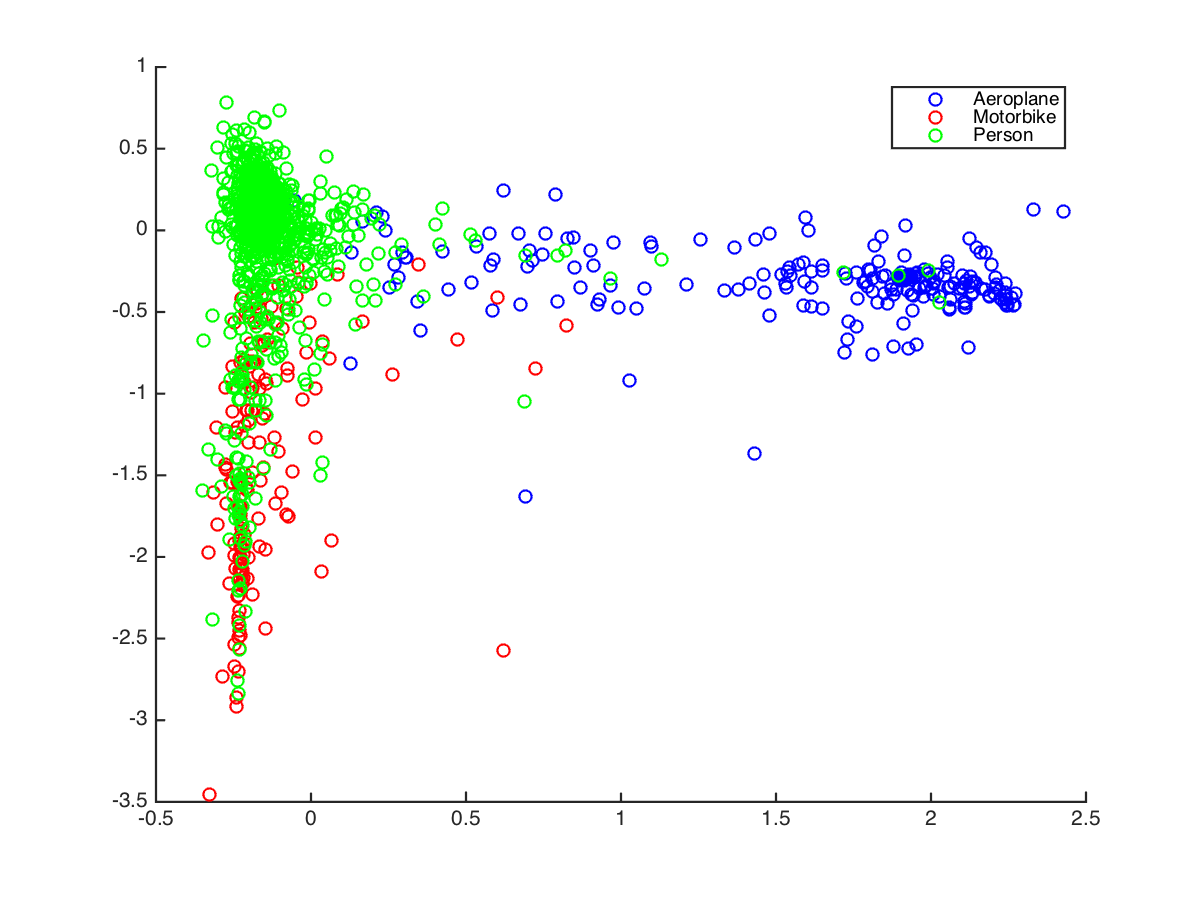
\includegraphics[width=\textwidth]{figures/toy1}
                \caption{ Canonical variates along the \textit{first two} directions; 'visual'.}
                \label{fig:1-toy}
        \end{subfigure}%
        ~ %add desired spacing between images, e. g. ~, \quad, \qquad, \hfill etc.
          %(or a blank line to force the subfigure onto a new line)
        \begin{subfigure}[b]{0.5\textwidth}
         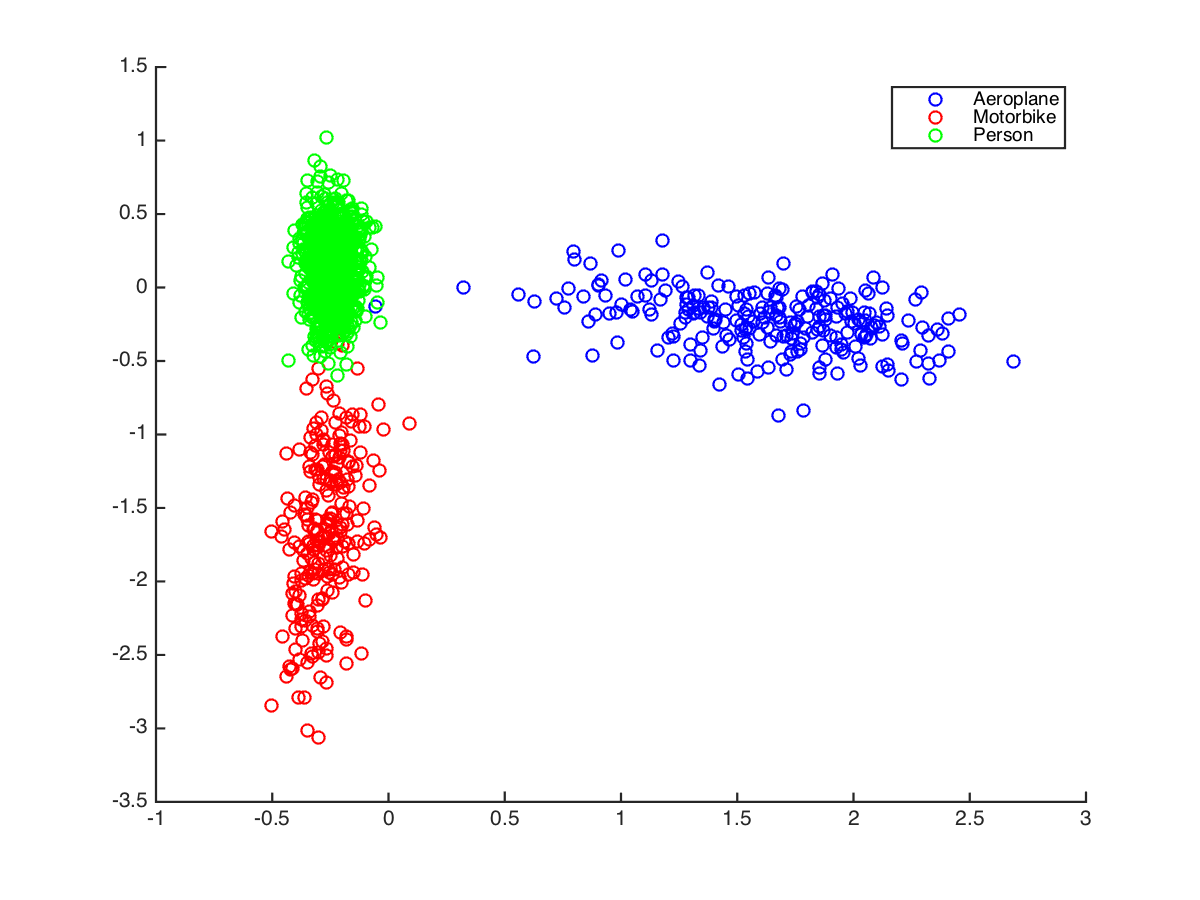
\includegraphics[width=\textwidth]{figures/toy1-bis}
                \caption{Canonical variates along the \textit{first two} directions; 'text'. }
                \label{fig:1-toybis}
        \end{subfigure}}
       %\caption{We find that the final clustering results are more or less similar and in all these three tests, the (normalized) distortion $j(\ct,z)$ stablizes at around $28.4$. We note that the cluster label depends on initialization.}
\label{fig:1-toys}
\end{figure} 

 \begin{figure}[H]
        \centering
              \makebox[0.6\textwidth][c]{         \begin{subfigure}[b]{0.5\textwidth}
 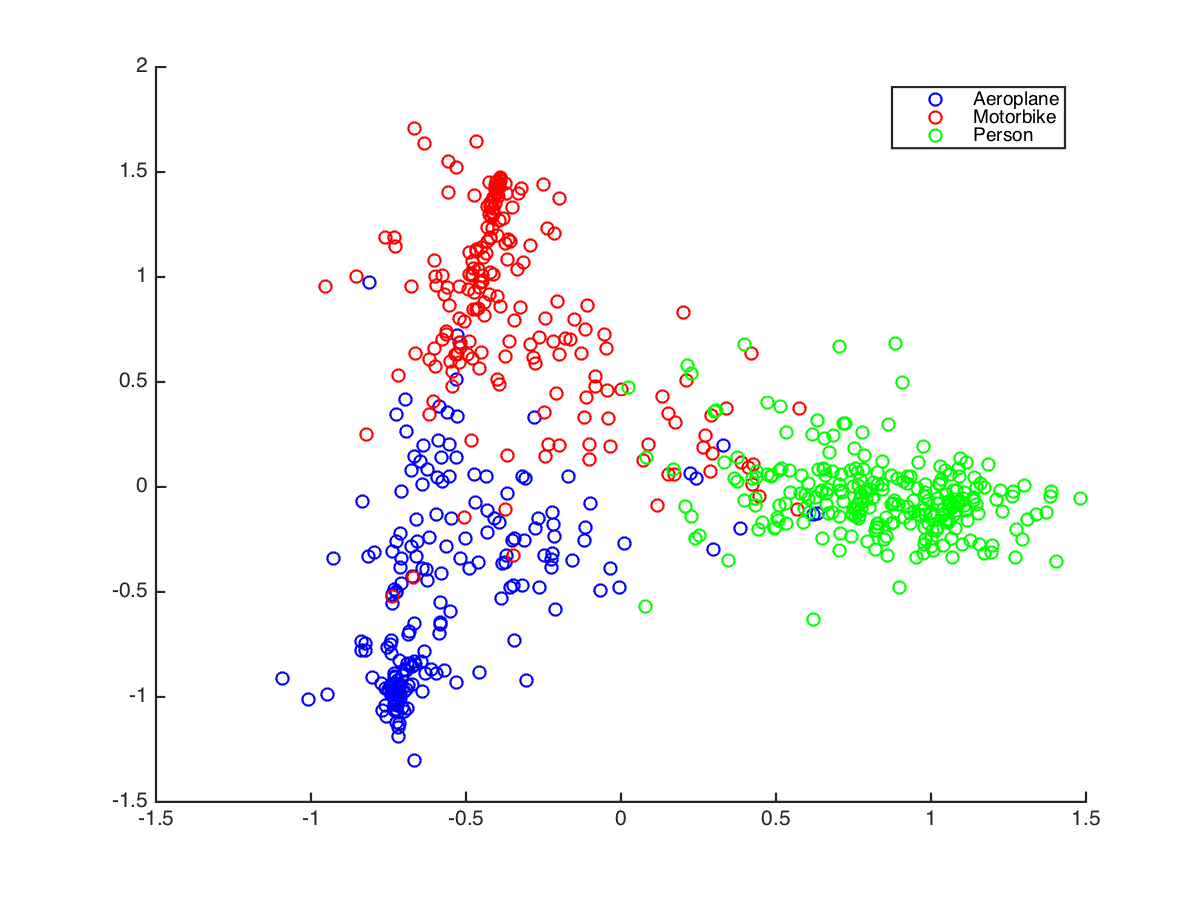
\includegraphics[width=\textwidth]{figures/13toy1}
                \caption{Canonical variates along directions 2 and 3 : $W_m(:,2)\text{ and } W_m(:,3)$; 'visual'.}
                \label{fig:1-toy23}
        \end{subfigure}%
        \begin{subfigure}[b]{0.5\textwidth}
         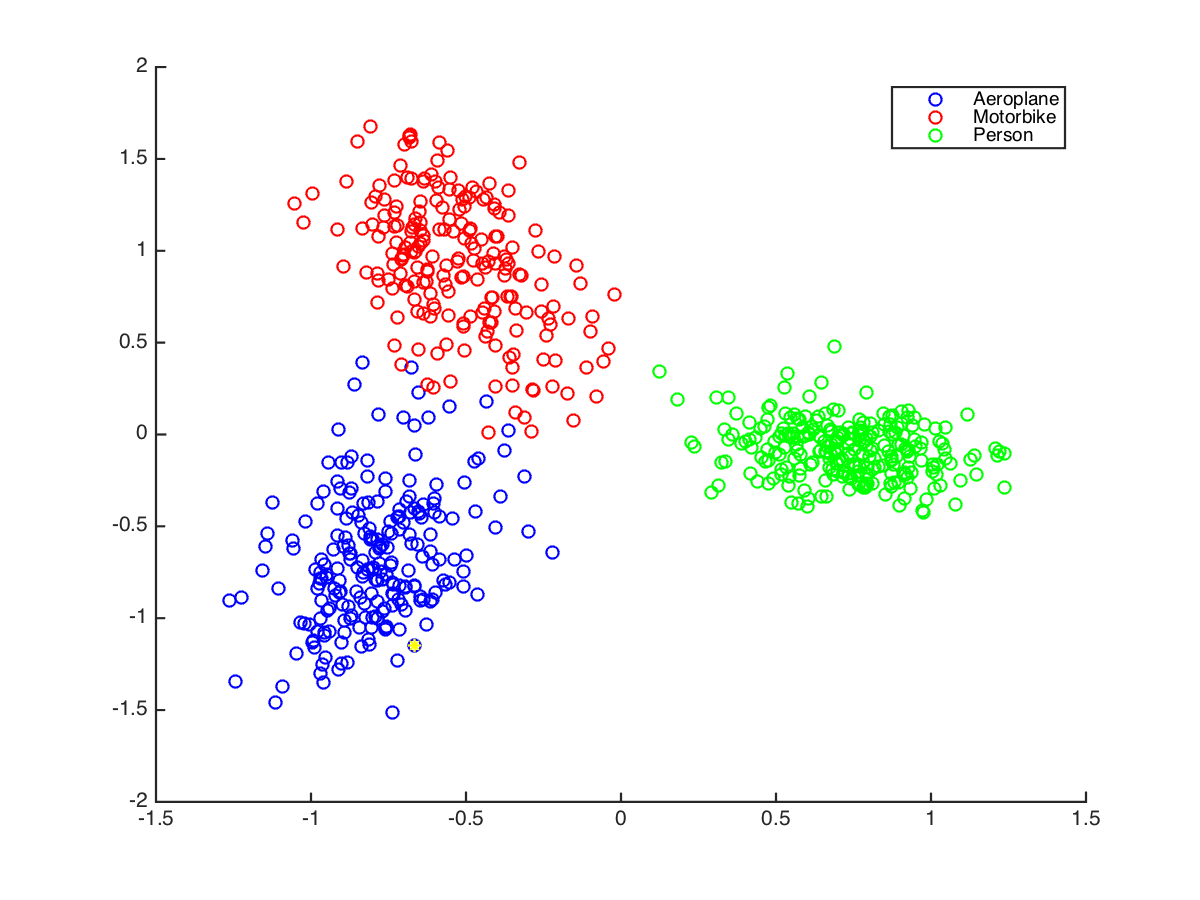
\includegraphics[width=\textwidth]{figures/13toy1-bis}
                \caption{Canonical variates along directions 2 and 3 : $W_m(:,2)\text{ and } W_m(:,3)$; 'text'. }
                \label{fig:1-toybis23}
        \end{subfigure}}
       %\caption{We find that the final clustering results are more or less similar and in all these three tests, the (normalized) distortion $j(\ct,z)$ stablizes at around $28.4$. We note that the cluster label depends on initialization.}
\label{fig:1-toys23}
\end{figure} 


\section{Dataset: INRIA-webqueries}

We will see in this section the characteristics of the dataset: INRIA-webqueries is composed of $71,748$ images, each image is related to one xml file containing information of the web page from which the image is downloaded.
The dataset is originated from 353 web search queries that represent various semantics such as tourist attractions, machines and objects, stars, sports, logos etc. Each of the $353$ classes is comprised of about $200 \sim 300$ images, some of which being irrelevant to the semantic, which is one source of the noise.

The \textbf{metadata} of each image is taken from the webpage and contains notably the title of the page and the texts surrounding the image (before and after it). We only use the text in these three fields to get text descriptions for each image. However, a non-negligeable proportion of these texts (not to mention those of other fields such as <imageURL> or <referer>) are irrelevant to the image content. As a result, INRIA-webqueries' text view has a source with greater noise compared to other datasets such as Pascal1K, Flickr8K, Flickr30K etc. 


\subsection{Visual feature}
The visual view is represented by CNN features of images using \textbf{Matconvnet}. The feature vector of the 20th and last layers of dimensions 4096 and 1000 are both tested as the visual feature.

We note that certain images ($4.74\%$ of all) do not have valid CNN representations due to their image file property (e.g. some of the images are actually in format \textbf{gif}). On the other hand, a very small percentage($0.51\%$) of images do not have text in neither of the three fields(<ptitle>, <before> and <after>).

Nevertheless, as these problems only represent $5.2\%$ of the total dataset, in the whole project we only consider the images that have valid CNN features and text descriptions at the same time, which represent $94.8\%$ of the dataset.

The following example shows the content of the dataset.
\begin{figure}[H]
\centering
\makebox[.4\textwidth][c]{         
 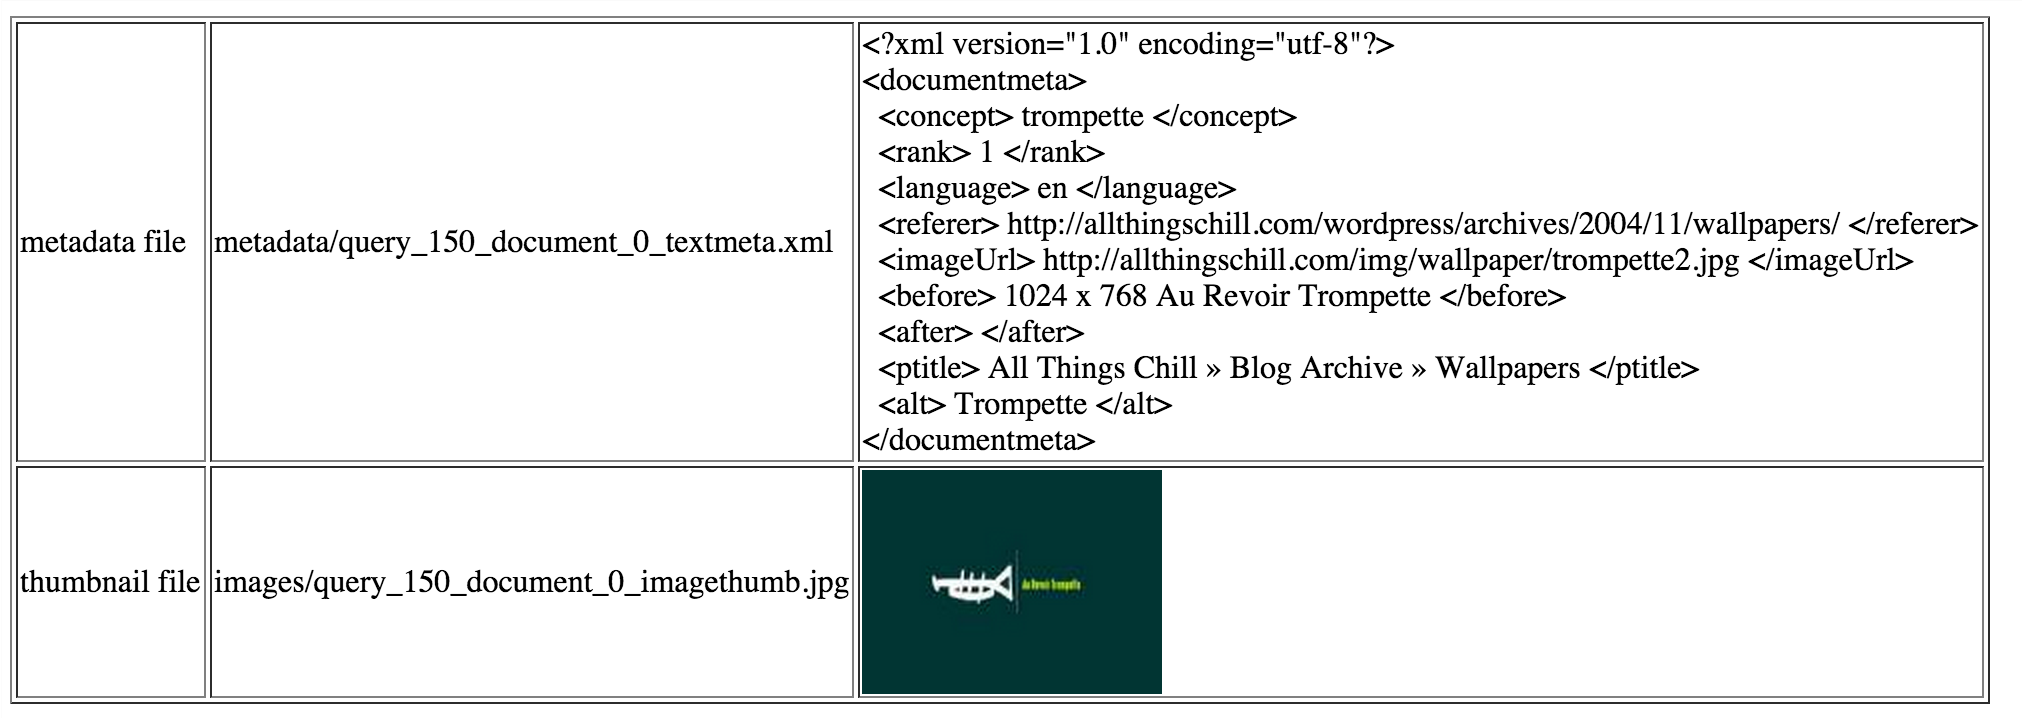
\includegraphics[width=1.1\textwidth]{figures/INRIAdataset}
 \label{fig:1-toy23}
 }
 \caption{For the text features, only text between (<ptitle>, </ptitle>), (<before>, </before>) and ((<after>, </after>)) are extracted.}
\label{fig:inria-dataset}
\end{figure} 


\subsection{Textual feature}
The text view is represented by vectors constructed from those of texts between <ptitle>, <before> and <after>; the vectors of these words come from a word-vector dictionary trained on the entire metadata using \textbf{word2vec}.

Precisely, for the nature of \textbf{metadata}, we only extract texts between (<ptitle>, </ptitle>), (<before>, </before>) and ((<after>, </after>)), \texttt{sed} and \texttt{awk} are used for this extraction. As a result, the entire text \texttt{inria\_text\_all.txt} of the metadata is the concatenation of all images' three text fields. We put this text file to train the dictionary with \textbf{word2vec}. The dictionary \texttt{dictionary\_inriaPBA.txt} contains $22,291$ word(s)-vector correspondances. The word vector is $200-$dimensional.

We notice that two words that have similar concepts or originated from the same context (in the original text) will lead to large cosine value between their vectors, thus the word2vec features provide useful and relevant representation for the text view.

As the textual feature depends almost totally on the word-vector dictionary trained by \textbf{word2vec}, which has two versions, one with only words and very few word combinaisons, and the other provides vectors for almost all highly frequent or correlated word combinations, such as \textit{"arc\_de\_triomphe", "mont\_blanc", "september\_11th"} etc. Therefore, two approaches of extracting textual features are tried with respect to these two versions of dictionaries.

\section{Training and test}


We take 4/5 of the total dataset as the training data and obtained the matrices containing $(w_x^k)$ and $(w_t^k)$, now we shall visualize the real canonical variates. There are $54,211$ training images/texts of 300 classes, we only show the data points of three classes of images/texts.



\begin{figure}[H]
        \centering
              \makebox[0.4\textwidth][c]{         \begin{subfigure}[b]{0.62\textwidth}
 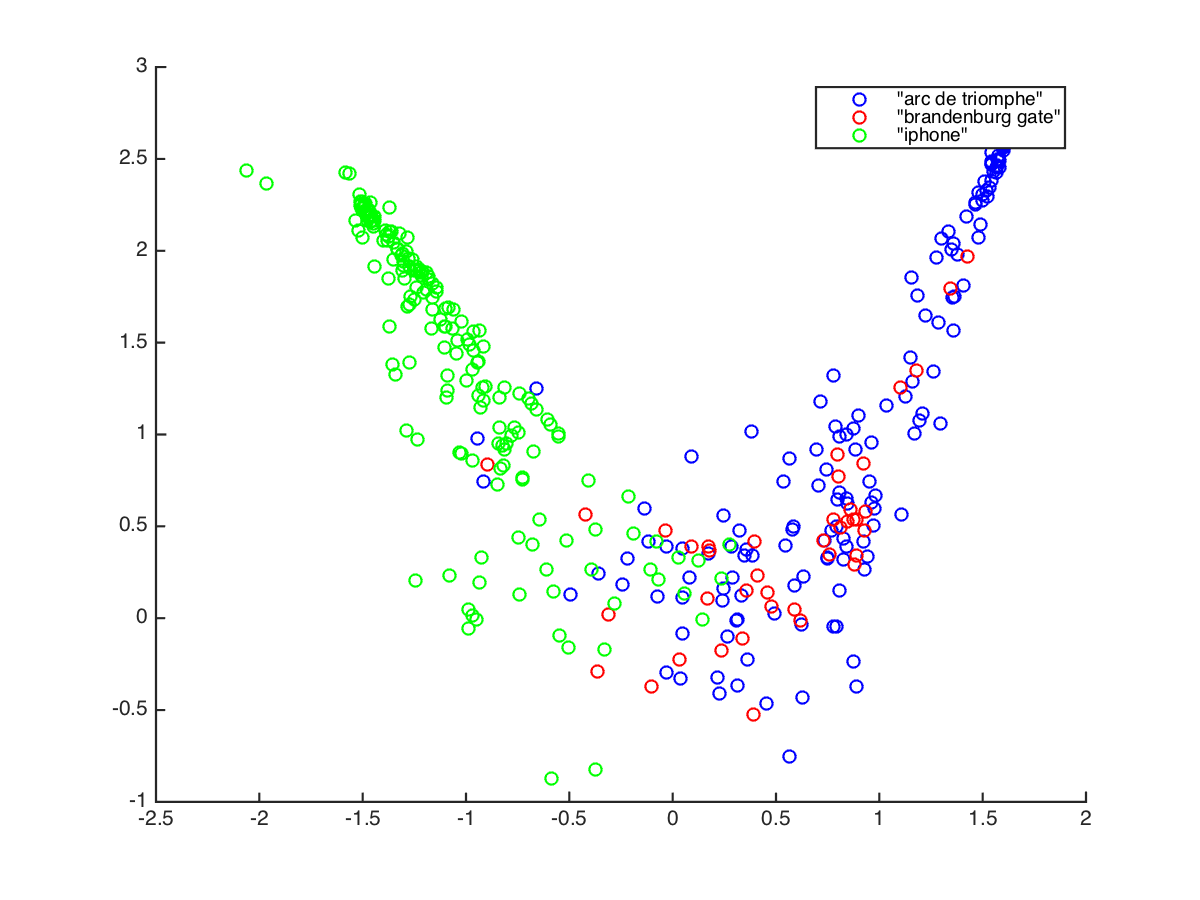
\includegraphics[width=\textwidth]{figures/v0-50-99}
                \caption{Canonical variates along directions 1 and 2:\\$W_m(:,1)\text{ and } W_m(:,2)$; 'visual'.}
                \label{fig:1-real23}
        \end{subfigure}%
        \begin{subfigure}[b]{0.62\textwidth}
         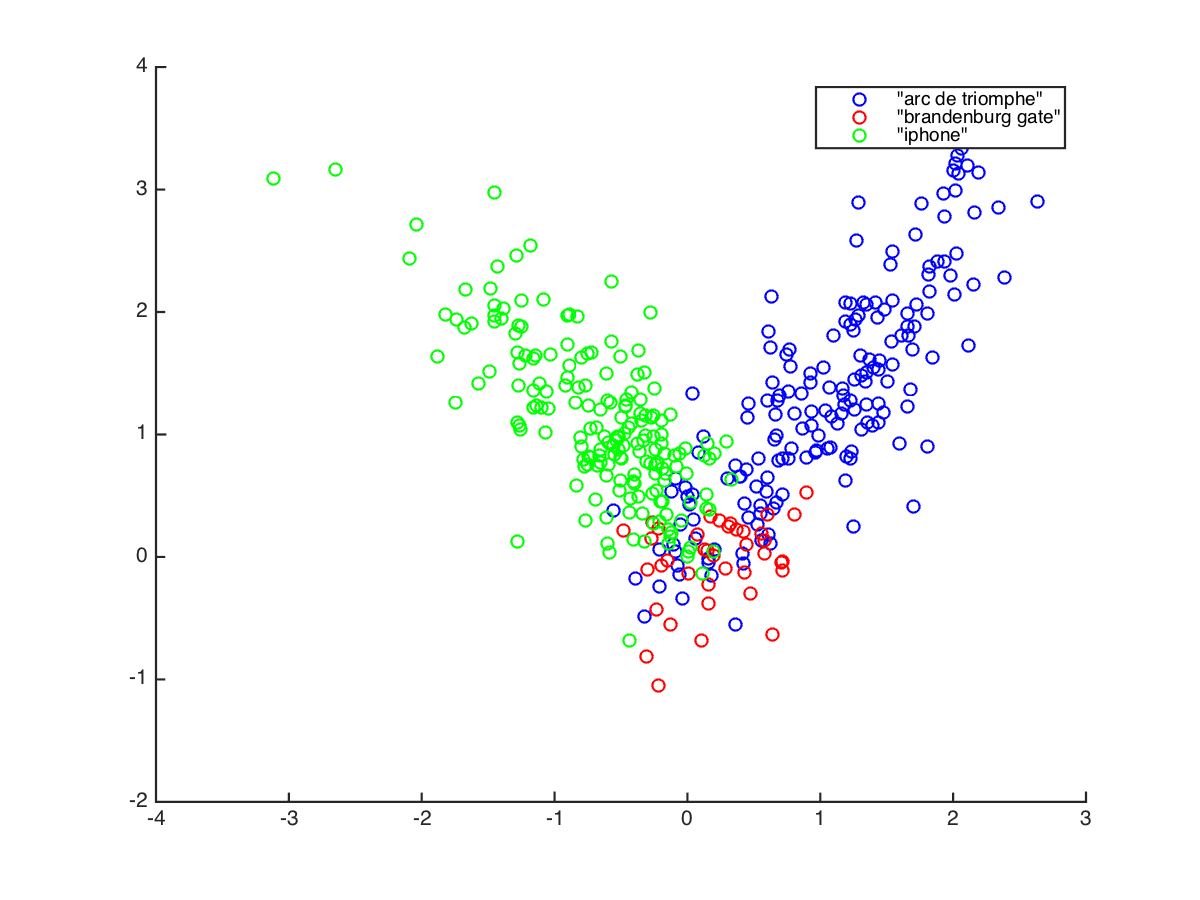
\includegraphics[width=\textwidth]{figures/t0-50-99}
                \caption{Canonical variates along directions 1 and 2:\\ $W_m(:,1)\text{ and } W_m(:,2)$; 'text'. }
                \label{fig:1-real23}
        \end{subfigure}}
       \caption{We notice that the projected points of \textit{arc de triomphe} and \textit{brandenburg gate} are difficult to be distinguished in the 'visual' view and that is easier in the 'textual' view. In both views, the clusters of \textit{arc de triomphe} and \textit{iphone} have two different directions.}
\label{fig:1-reall23}
\end{figure} 


One important parameter for the retrieval tasks is the number $d$ of top ranked eigen-vectors $(w_m^k)_{k=1,..,d} = W_m$, for $m = x \text{ (visual) }$ and $t\text{ (textual) }$. The cosine similarity measure in the latent space depends much on this dimensionality:

$$ S(x,t) = \frac{ ( W_x^{\ts}\varphi(x))^{\ts}(W_t^{\ts}\varphi(t))} {\Vert W_x^{\ts}\varphi(x) \Vert_2 \Vert W_t^{\ts}\varphi(t) \Vert_2}.
$$
We notice that it is equivalent to the similarity meaure defined in \citep{cca0} in case the p-th power is set to $1$. The measure $S$ between the visual view $x$ and the textual view $t$ will be extended naturally to that within the visual view (for image-to-image retrival). 

We visualize some of the image-text retrieval examples on test data using the above similarity measure.

\subsection{Image-to-text search on test data}

We carry out the image-to-text search on the remaining test data and visualize the results of several images

\begin{figure}[H]
\centering
\makebox[.4\textwidth][c]{         
 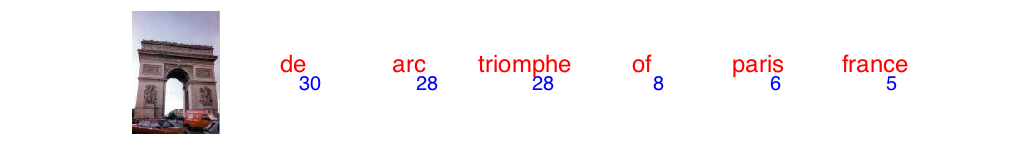
\includegraphics[width=1.1\textwidth]{figures/I2T-arc1}
 \label{fig:1-arc1}
 }
% \caption{}
\label{fig:inria-dataset}
\end{figure} 

\begin{figure}[H]
\centering
\makebox[.4\textwidth][c]{         
 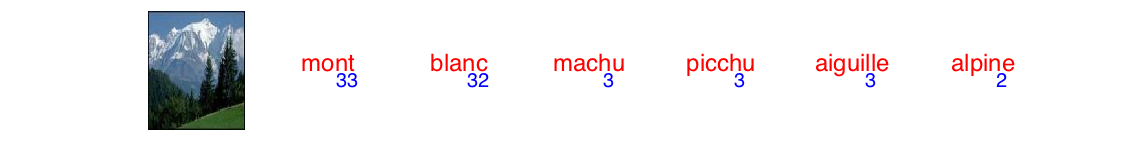
\includegraphics[width=1.1\textwidth]{figures/I2T-montb1}
 \label{fig:1-arc1}
 }
% \caption{}
\label{fig:inria-dataset}
\end{figure} 

\begin{figure}[H]
\centering
\makebox[.4\textwidth][c]{         
 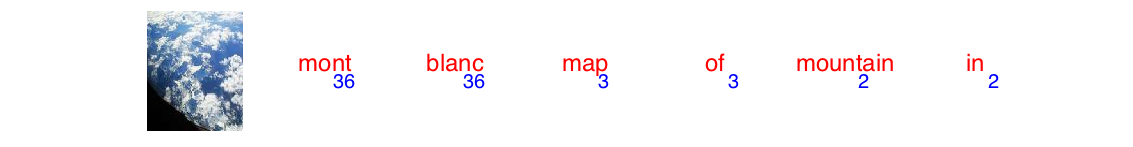
\includegraphics[width=1.1\textwidth]{figures/I2T-montb2}
 \label{fig:1-arc1}
 }
% \caption{}
\label{fig:inria-dataset}
\end{figure} 

\begin{figure}[H]
\centering
\makebox[.4\textwidth][c]{         
 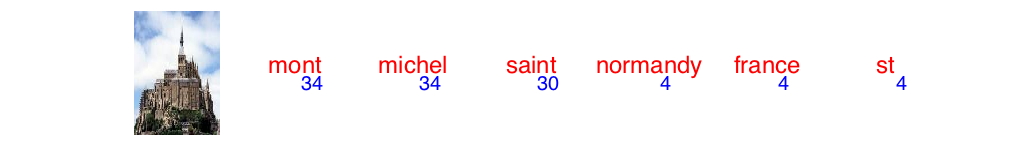
\includegraphics[width=1.1\textwidth]{figures/I2T-monts1}
 \label{fig:monts1}
 }
 %\caption{Four examples of image-to-text search on test data.}
\label{fig:i2t}
\end{figure} 


\begin{figure}[H]
\centering
\makebox[.4\textwidth][c]{         
 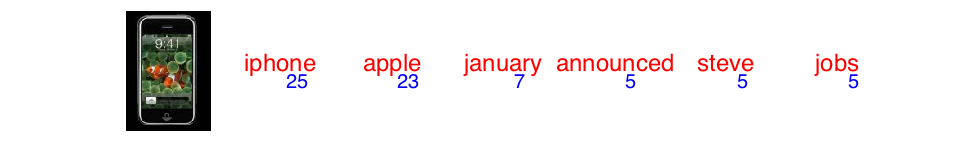
\includegraphics[width=1.1\textwidth]{figures/I2T-apple135}
 \label{fig:1-arc1}
 }
 \caption{Five examples of image-to-text search on test data: the words correspond to the trained text vectors that have the highest similarities with the test image's visual feature; the scores is the count of occurrences of such each word.}
\label{fig:i2t}
\end{figure} 


%\subsection{Image-to-image search on test data}

For three images in the figure (\ref{fig:i2t}) and we visualize the images in training set that correspond to the top ranked texts:

%%
\begin{figure}[H]
\centering
\makebox[.4\textwidth][c]{         
 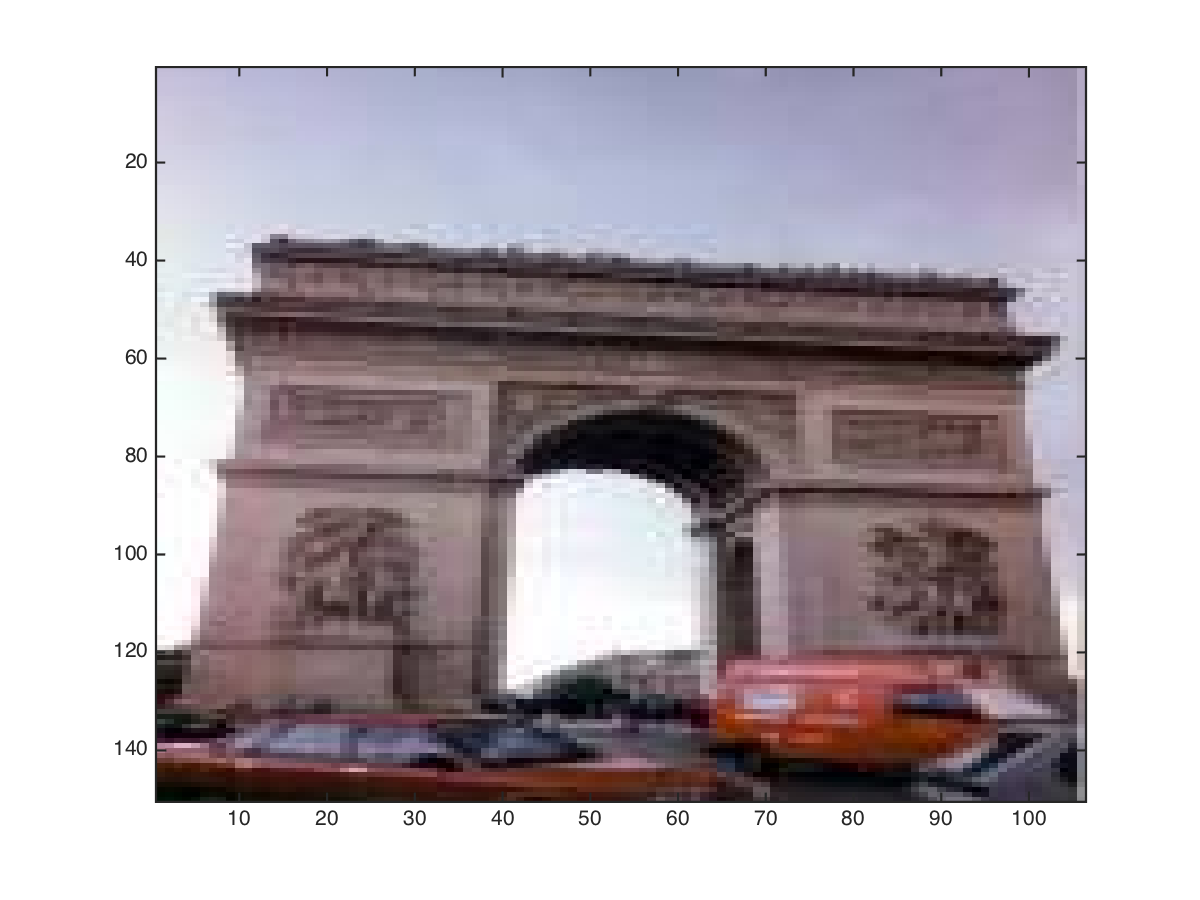
\includegraphics[width=0.15\textwidth]{figures/I2I-arc1all-r}
 \label{fig:i2iappler}
 }
  %\caption{}
\label{fig:inria-dataset}
\end{figure} 

\begin{figure}[H]
\centering
\makebox[.4\textwidth][c]{         
 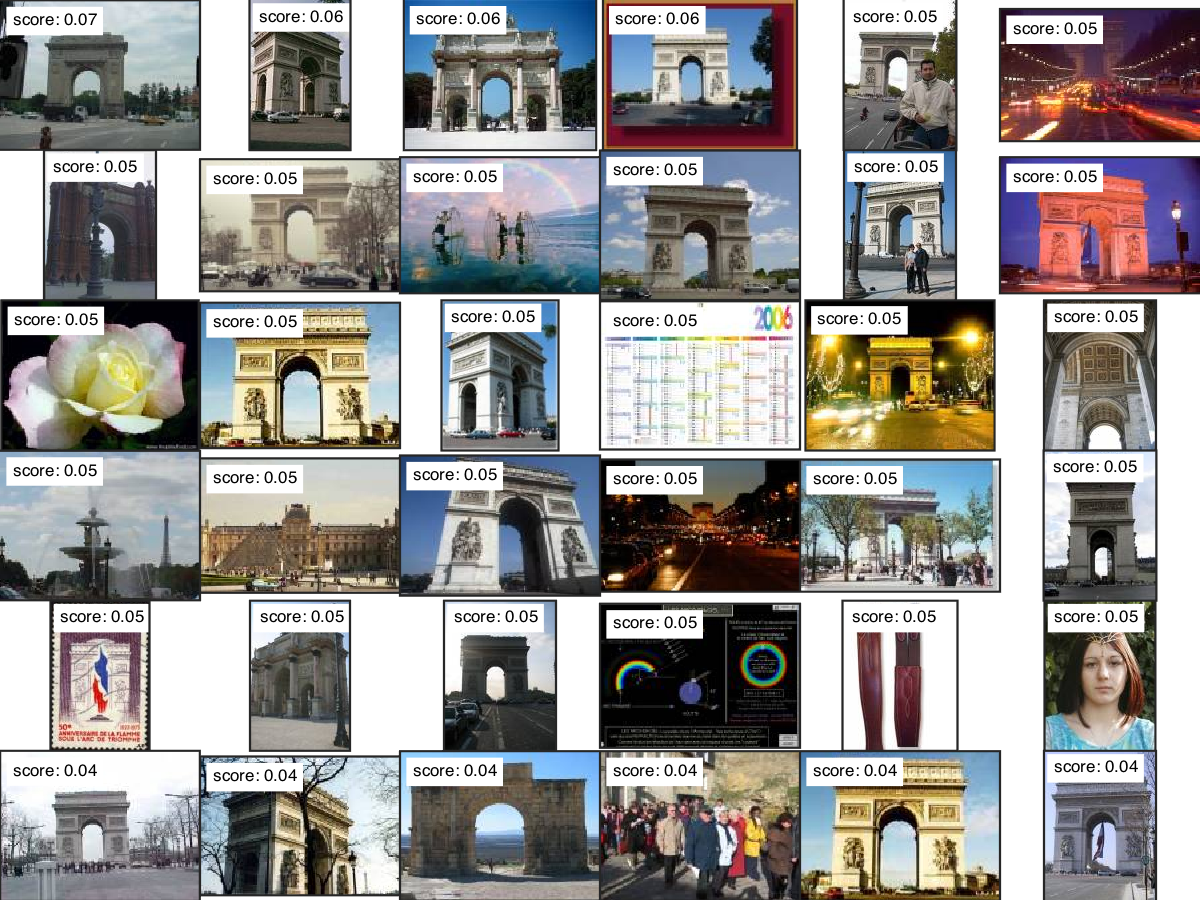
\includegraphics[width=1\textwidth]{figures/I2I-arc1all}
 \label{fig:i2iapple1}
 }
% \caption{}
\label{fig:inria-dataset}
\end{figure} 
%%
\begin{figure}[H]
\centering
\makebox[.4\textwidth][c]{         
 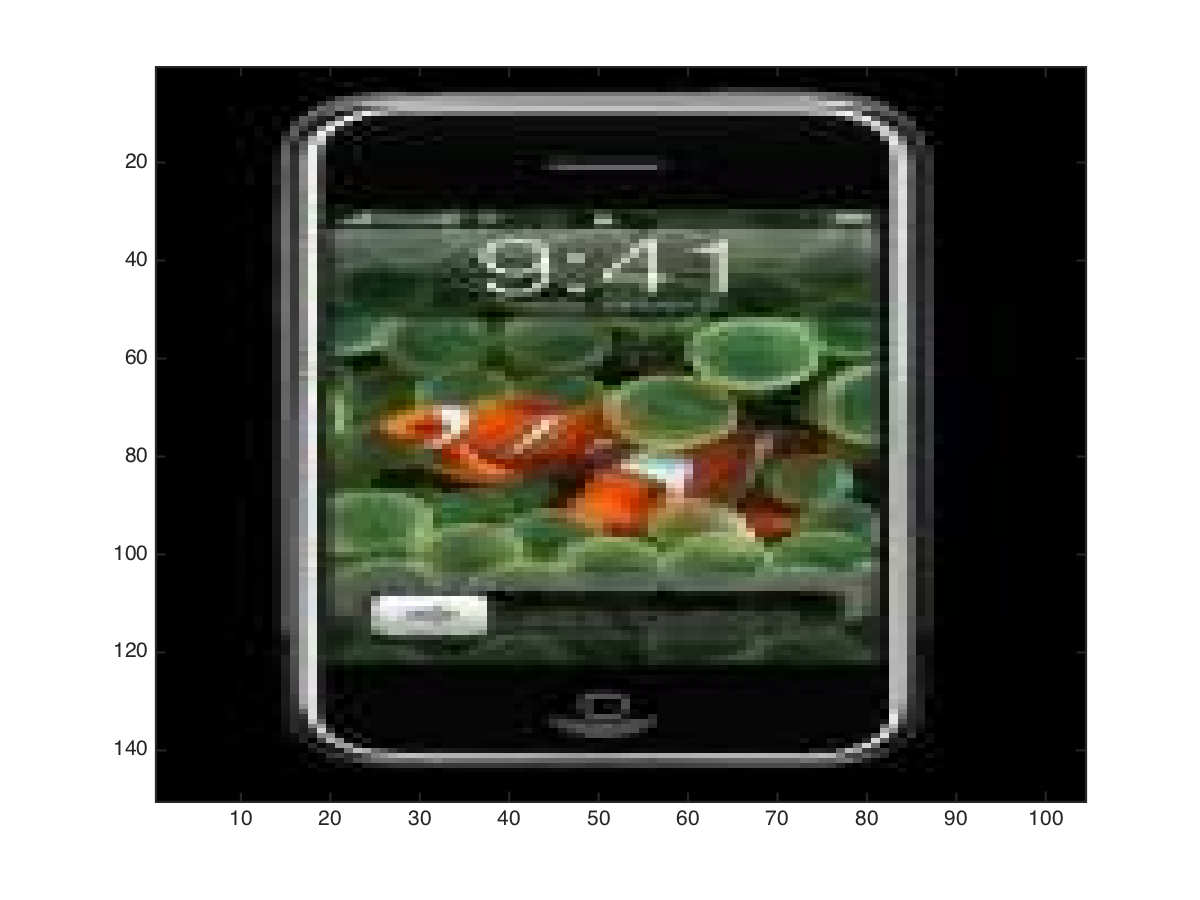
\includegraphics[width=0.15\textwidth]{figures/I2I-apple1all-r}
 \label{fig:i2iappler}
 }
  %\caption{}
\label{fig:inria-dataset}
\end{figure} 

\begin{figure}[H]
\centering
\makebox[.4\textwidth][c]{         
 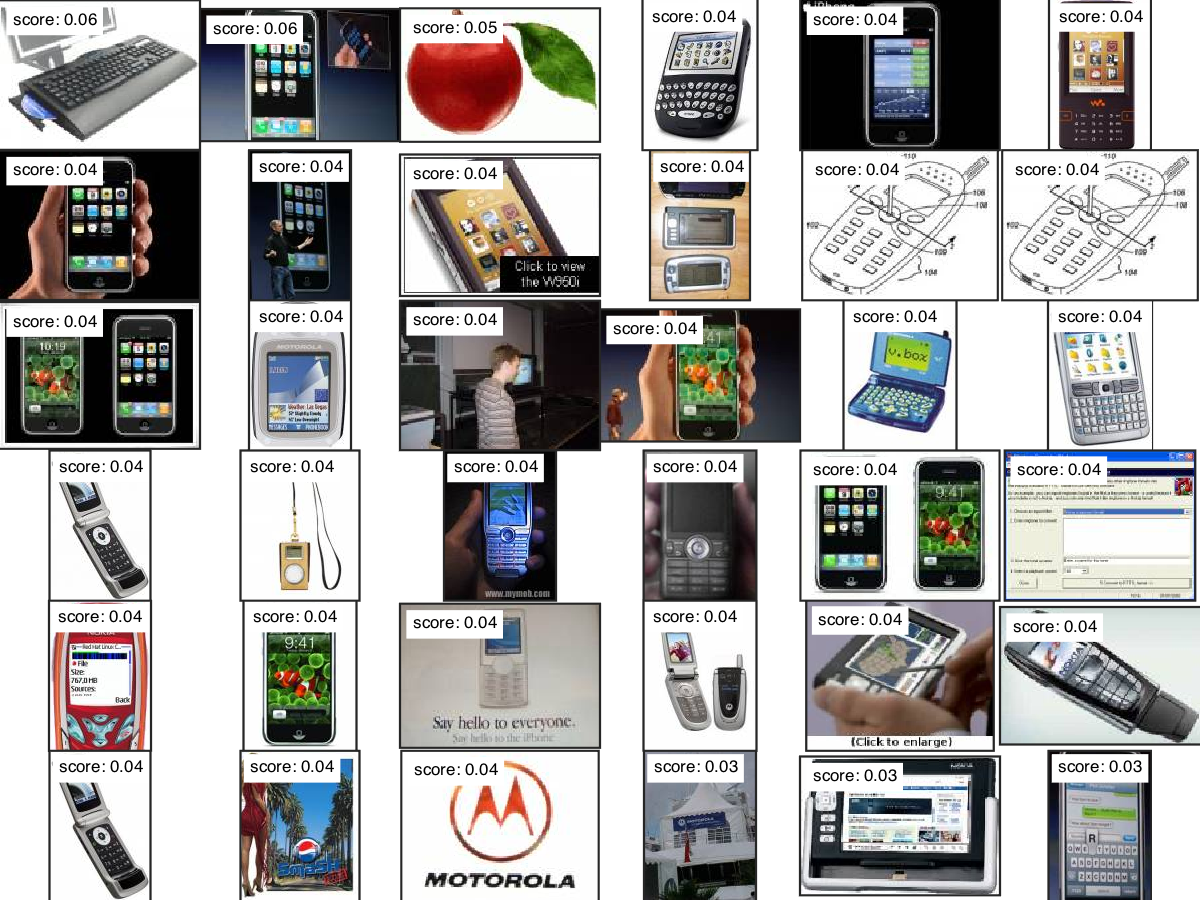
\includegraphics[width=1\textwidth]{figures/I2I-apple1all}
 \label{fig:i2iapple1}
 }
% \caption{}
\label{fig:inria-dataset}
\end{figure} 

%\begin{figure}[H]
%\centering
%\makebox[.4\textwidth][c]{         
% 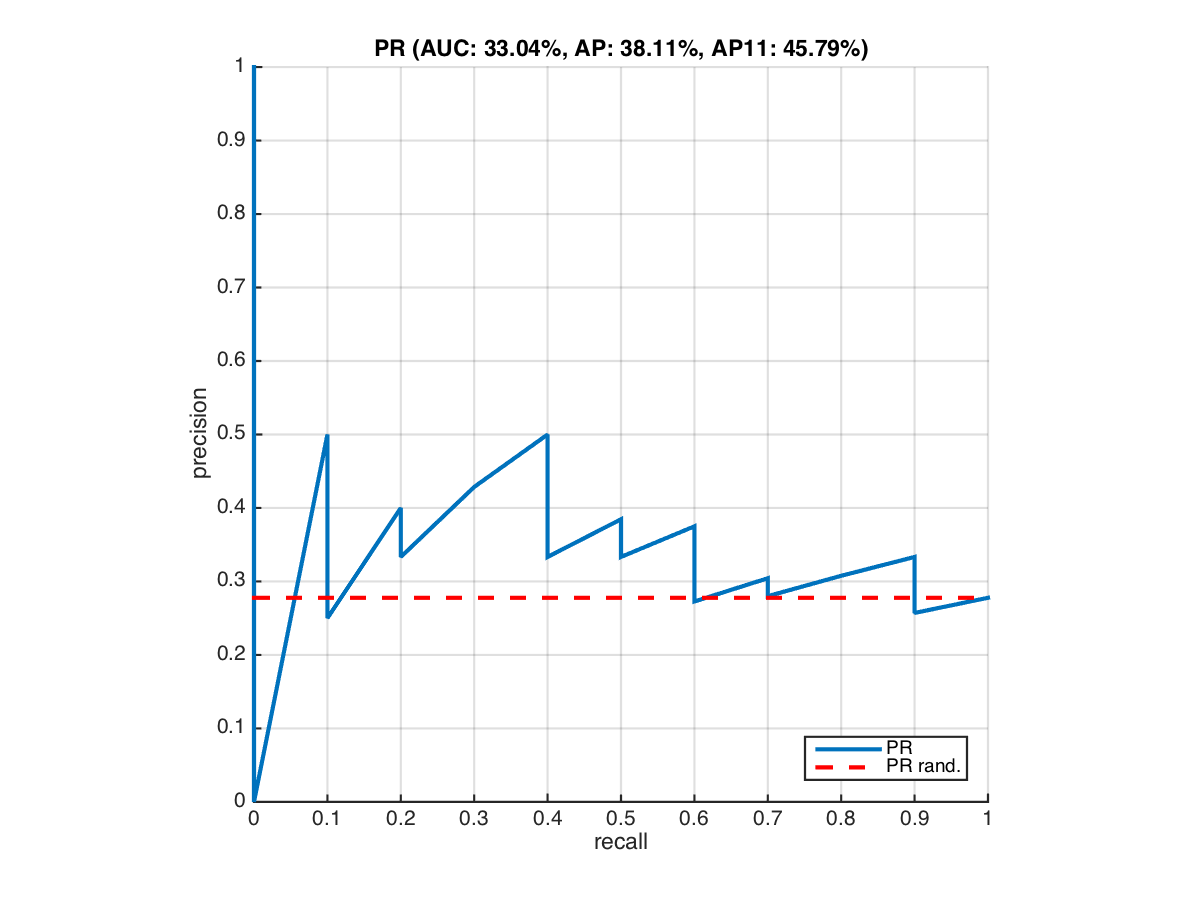
\includegraphics[width=0.7\textwidth]{figures/I2I-APR-apple1all}
% \label{fig:i2iapple1apr}
% }
    % \caption{}
%\label{fig:i2iapple}
%\end{figure} 
%% monts1

\begin{figure}[H]
\centering
\makebox[.4\textwidth][c]{         
 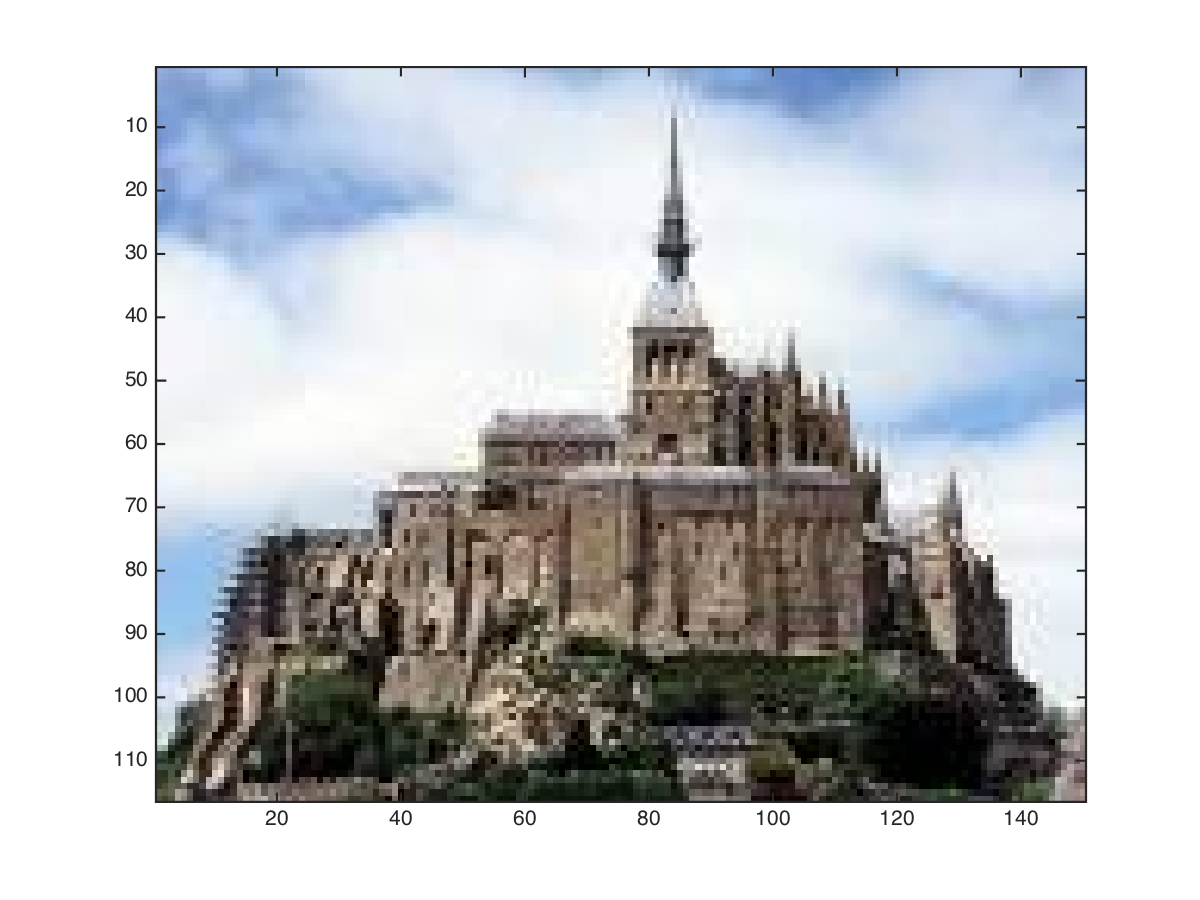
\includegraphics[width=0.15\textwidth]{figures/I2I-monts1all-r}
 \label{fig:i2iappler}
 }
 \caption{}
\label{fig:inria-dataset}
\end{figure} 

\begin{figure}[H]
\centering
\makebox[.4\textwidth][c]{         
 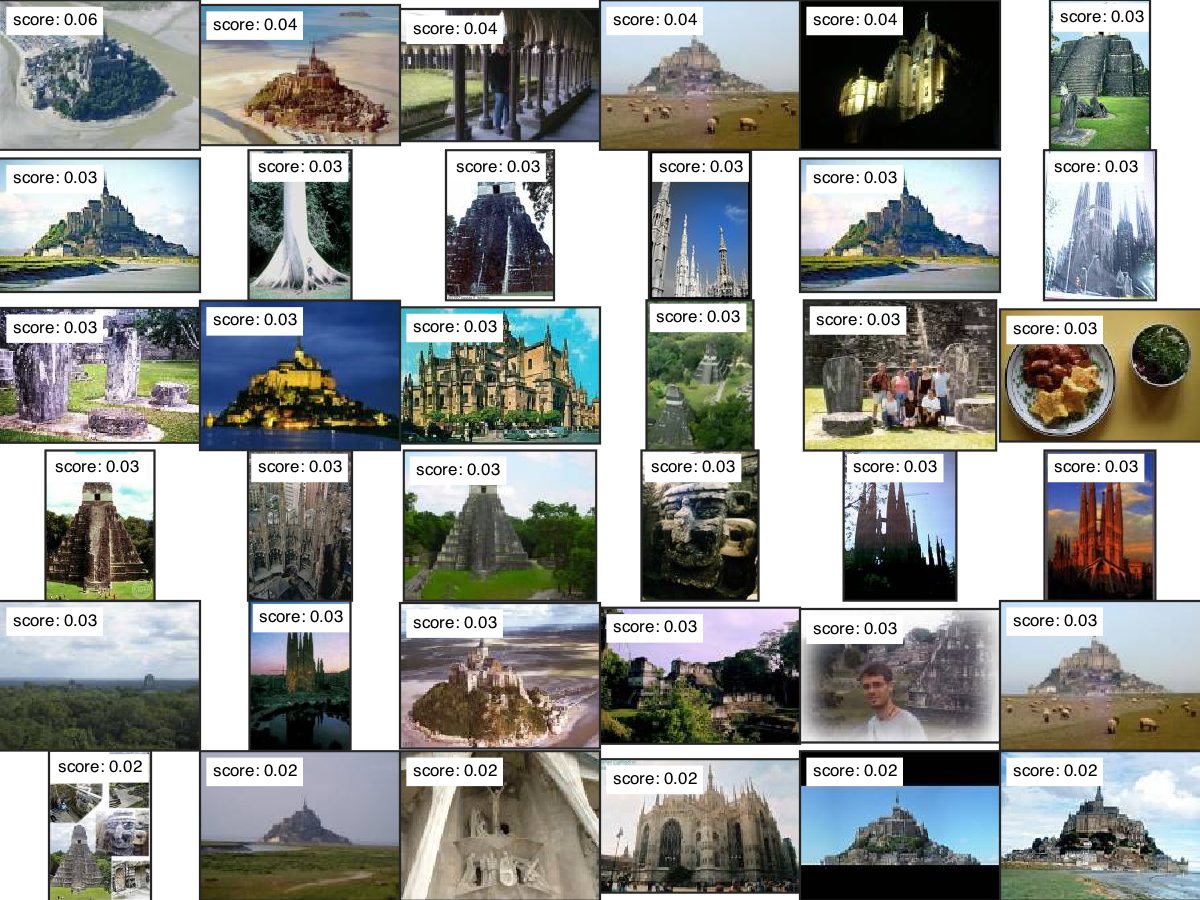
\includegraphics[width=1\textwidth]{figures/I2I-monts1all}
 \label{fig:i2iapple1}
 }
% \caption{}
\label{fig:inria-dataset}
\end{figure} 

%\begin{figure}[H]
%\centering
%\makebox[.4\textwidth][c]{         
% 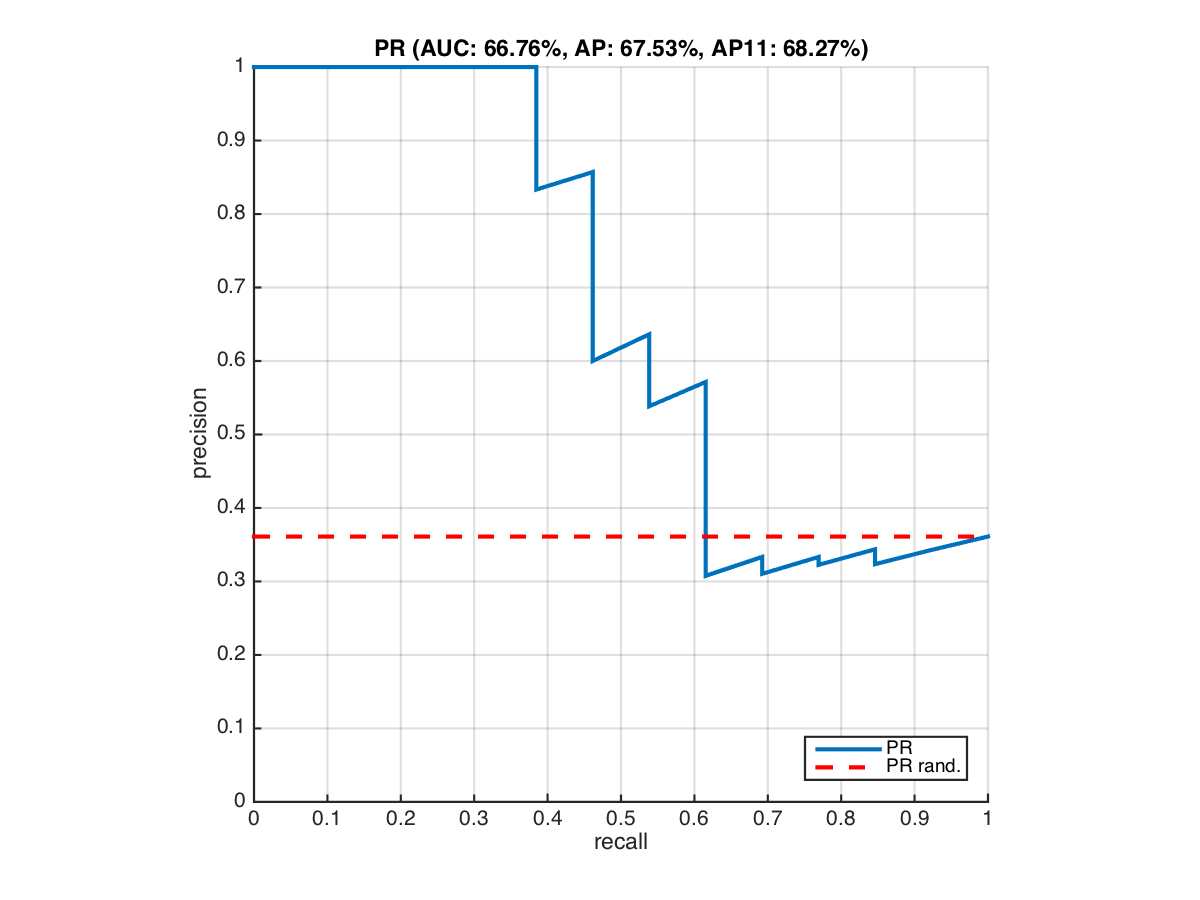
\includegraphics[width=0.8\textwidth]{figures/I2I-APR-monts1all}
% \label{fig:i2iapple1apr}
% }
% \caption{Precision-recall curve for test image: mont saint michel}
%\label{fig:i2iapple}
%\end{figure} 

\subsection{Text-to-image search on test data}
We carry out the text-to-image search on the same test data and visualize the top ranked images:


By typing the follwoing texts, we have: 

" metro paris plan": 
\begin{figure}[H]
\centering
\makebox[.4\textwidth][c]{         
 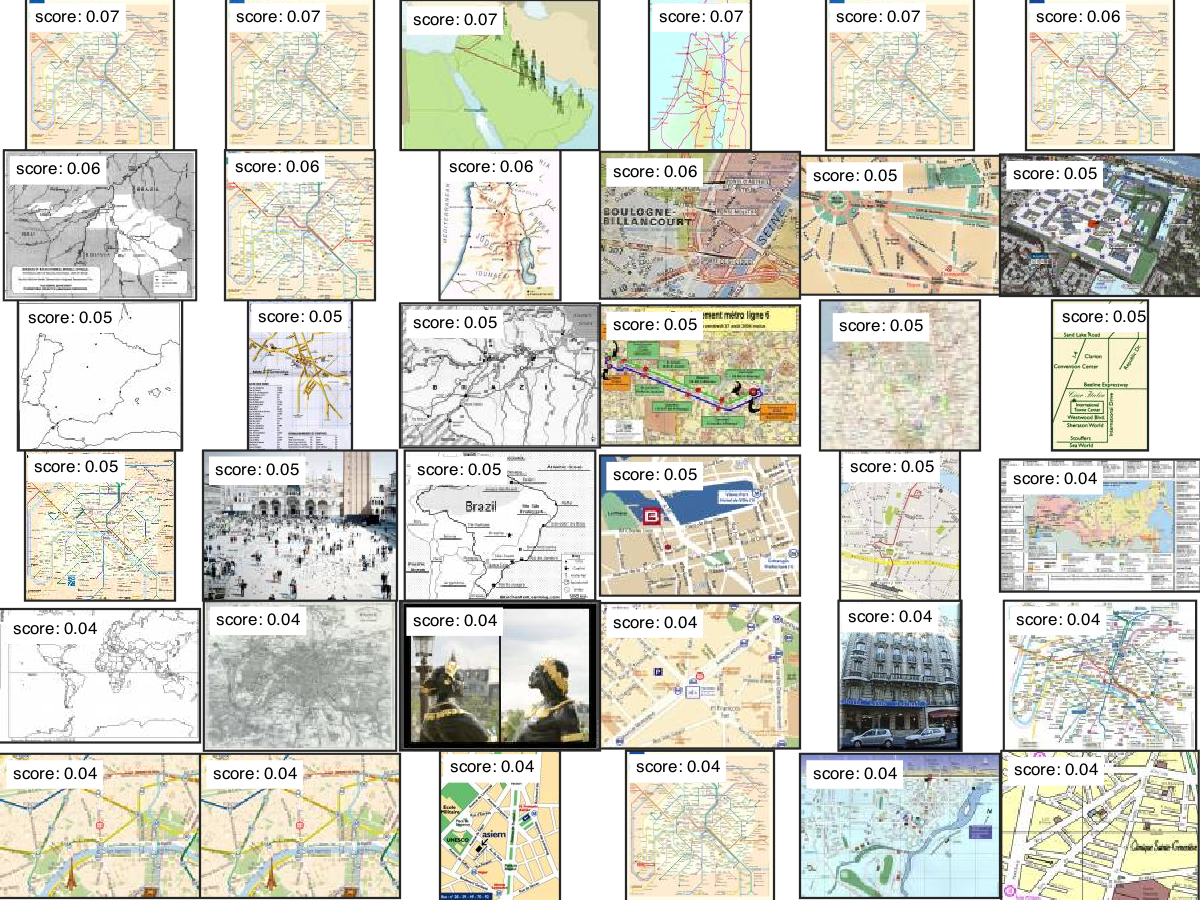
\includegraphics[width=1.1\textwidth]{figures/ranksT2I-metroparis}
 \label{fig:1-metro}
 }
% \caption{}
\label{fig:inria-dataset}
\end{figure} 

And "mont blanc":

\begin{figure}[H]
\centering
\makebox[.4\textwidth][c]{         
 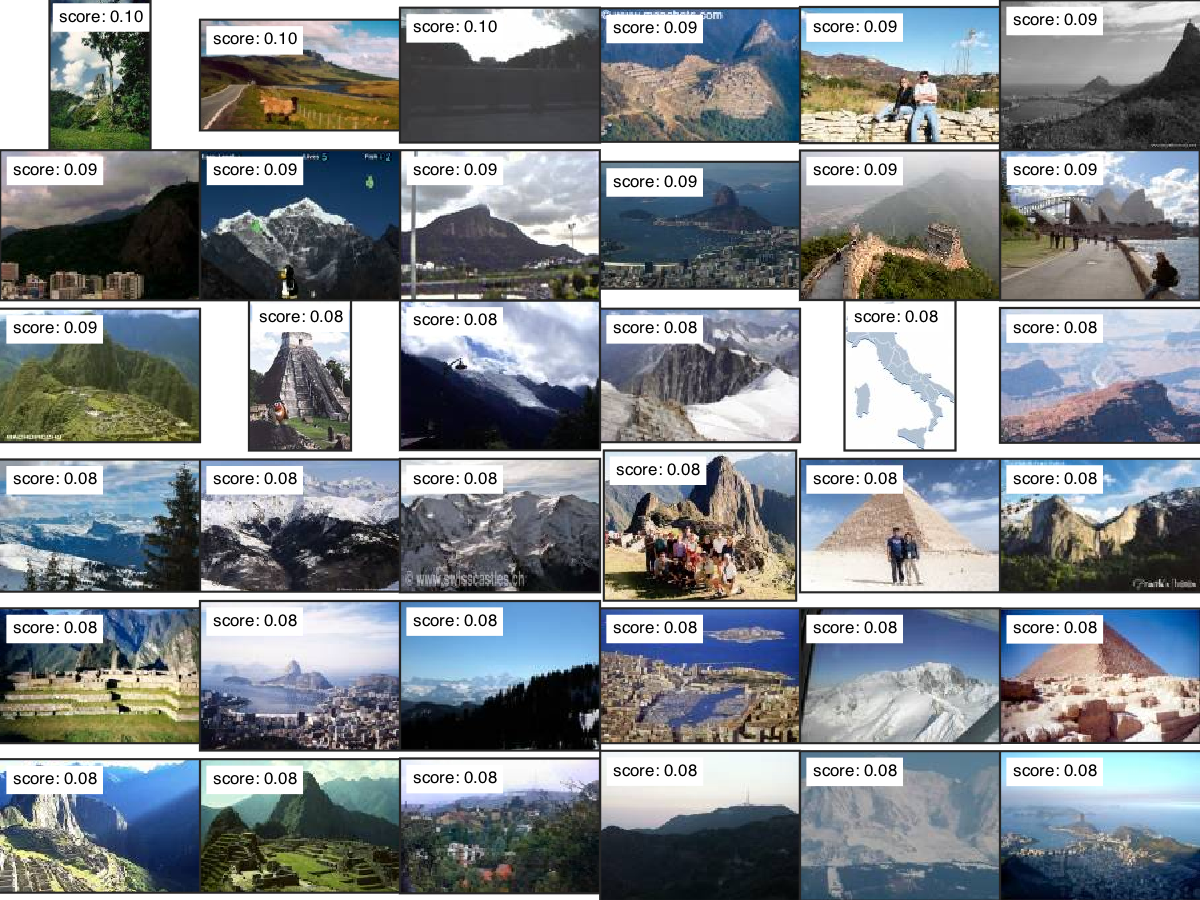
\includegraphics[width=1.1\textwidth]{figures/ranksT2I_periodic}
 \label{fig:1-metro}
 }
% \caption{}
\label{fig:inria-dataset}
\end{figure} 


\section{Evaluations and conclusion}
 
\bibliographystyle{agu04}
\footnotesize
\bibliography{biblio}
\normalsize




\end{document}
%%% Fin du document %%%
	
